\chapter{Assurance Cases and Selected Evidence for AortaGeomRecon}

\section{Assurance Case Development}

\section{Assurance Case for Software Specification Requirements}

\begin{itemize}
\item \citep{SRS}
\item Goals
\item Assumptions
\item Data Definitions
\item Instance Model
\item Functional Requirements
\item Non-Functional Requirements
\item Traceability Matrix Between Different Sections
\item Traceability Matrix Between Requirements and Other Sections
\end{itemize}

\section{Assurance Case for Implementation}
\begin{itemize}
\item Design Document
\begin{itemize}
\item Sphinx - Python Documentation Generator
\item Comments in the source code
\item Algorithm Overview - Explanation and Program Workflow
\item Glossary
\end{itemize}
\item Module Guide
\begin{itemize}
\item Traceability Matrix between Modules and Requirements
\item Traceability Matrix between Modules and Source Code
\end{itemize}

\item Test Case
\begin{itemize}
\item GitHub Workflow
\item Continuous Integration tests
\begin{itemize}
\item build ``Ground Truth Data''
\item Steps
\item Coverage
\end{itemize}
\end{itemize}

\end{itemize}

\section{Algorithm Review}
\begin{itemize}
\item Python Spyder IDE - Data Visualization and Debugging tool
\item Algorithm Review with Kailin Chu
\item Algorithm Review with Dr. Dean Inglis
\end{itemize}


%\section{Referencing}
%These are some sample references to GAMYGDALA~\citep{popescu2014gamygdala} from 
%the \texttt{references.bib} file and state effects of 
%cognition~\citep{hudlicka2002time} from the \texttt{references\_another.bib} 
%file. These references are not in the same .bib file.
%
%\section{Figures}
%This is a single image figure (Figure~\ref{fig_singleenv}):
%
%\begin{figure}[ht]
%    \centering
%    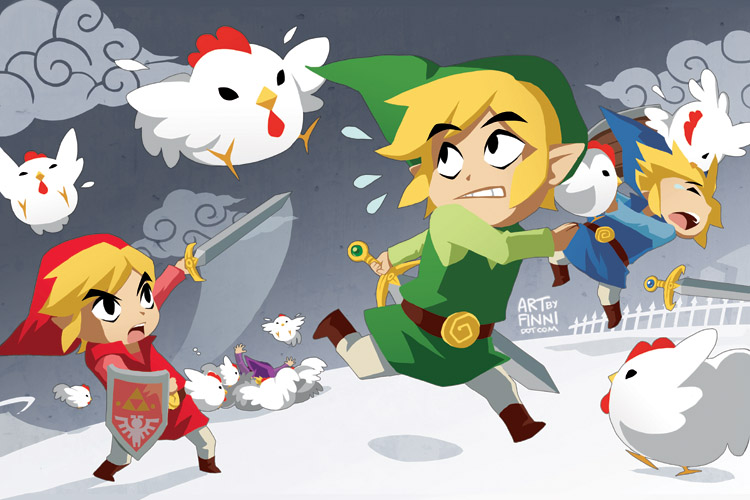
\includegraphics[width=0.6\textwidth]{figures/Sample/tumblr_static_eaceks0rfxsss8o4swscw40wo.jpg}
%    \caption[Single Figure Environment Listed Title]{This is a single figure 
%    environment}
%    \label{fig_singleenv}
%\end{figure}
%
%This is a multi-image figure with a top (Figure~\ref{fig_multienv_1}) and bottom (Figure~\ref{fig_multienv_2}) aligned subfigures:
%
%\begin{figure}[ht]
%	\centering
%	\begin{subfigure}[t]{\textwidth}
%		\centering
%		
%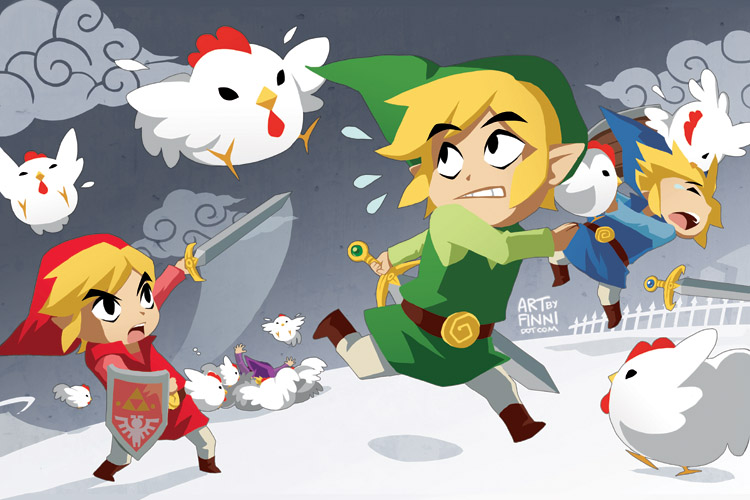
\includegraphics[width=0.7\textwidth]{figures/Sample/tumblr_static_eaceks0rfxsss8o4swscw40wo.jpg}
%		\caption{Figure 1}
%		\label{fig_multienv_1}
%	\end{subfigure}
%	~
%	\begin{subfigure}[t]{\textwidth}
%		\centering
%		
%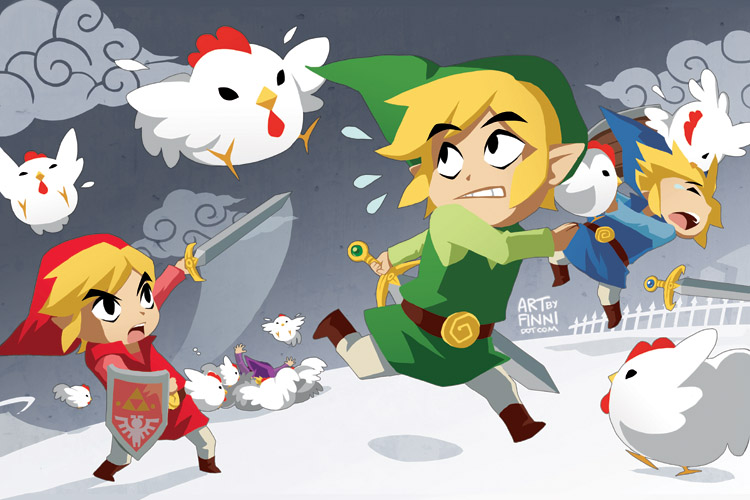
\includegraphics[width=0.7\textwidth]{figures/Sample/tumblr_static_eaceks0rfxsss8o4swscw40wo.jpg}
%		\caption{Figure 2}
%		\label{fig_multienv_2}
%	\end{subfigure}
%	
%	\caption{A Multi-Figure Environment}
%	\label{fig_multienv}
%\end{figure}
%
%\section{Tables}
%
%Here is a sample table (Table~\ref{tab_sample}):
%
%	\begin{table}[ht]
%	\centering
%	\begin{tabular}{ m{0.2\textwidth} m {0.1\textwidth} m{0.15\textwidth} }
%		\toprule
%		A & $\longleftrightarrow$ & B \\
%		C & $\longleftrightarrow$ & D \\
%		\bottomrule	
%	\end{tabular}	
%	\caption{A sample table}	
%	\label{tab_sample}
%\end{table}
%
%\subsection{Long Tables}
%A sample long table is shown in Appendix~\ref{appendix_b}.
%
%\section{Equations}
%
%Here is a sample equation (Equation~\ref{eq_lineslope}):
%
%\begin{equation} \label{eq_lineslope}
%	y = mx + b
%\end{equation}